%-------------------------------------------------------------------------------
%-------------------------------------------------------------------------------
\section{Déterminant} \label{sec:LinAlg-Det}
%-------------------------------------------------------------------------------
%-------------------------------------------------------------------------------

\begin{definition}[Matrice inversible] \label{def:matriceInversible}
  Une matrice $A \in \Mcal_n$ est dite inversible si la solution $x \in \Rbb^n$ du système linéaire $A x = y$ est unique quelque soit le vecteur $y \in \Rbb$.
\end{definition}

Il existe alors une unique matrice $B$ telle que 
$$
AB = BA = I_n
$$
et notée $A^{-1} = B$. La solution de $Ax = y$ est alors $x = A^{-1} y$.

\bigskip
On cherche à déterminer à quelle condition une matrice carrée $A$ est inversible.

%-------------------------------------------------------------------------------
%-------------------------------------------------------------------------------
\subsection{Matrices $2 \times 2$} 
%-------------------------------------------------------------------------------

\paragraph*{Exemple.}
Une condition nécessaire et suffisante sur $(a, b, c, d)$ pour que 
$$
A = \left[\begin{array}{cc} a & b \\ c & d \end{array} \right]
$$
soit inversible est que 
$$
ad - bc \neq 0
$$
(il suffit de résoudre le système $A x  = y$). Son inverse est alors
$$
A^{-1} = \frac1{ad - bc} \left[\begin{array}{rr} d & -b \\ -c & a \end{array}\right].
$$

\solution{Voir \cite{Lam20}, p 6.}

\begin{definition}[1.2.2: Déterminant d'une matrice de $\Mcal_2$] \label{def:determinantMatrice22}
  Le déterminant de la matrice $A \in \Mcal_2$ est noté $\det(A)$ ou $|A|$ et vaut
  $$
  |A| = a_{11} a_{22} - a_{12} a_{21}.
  $$
\end{definition}

\bigskip
Le déterminant d'une matrice de $\Mcal_2$ est une fonction continue qui s'annule ssi la matrice n'est pas inversible : on cherche à généraliser cette notion aux matrices de $\Mcal_n$.

\remark
On vérifie facilement que le déterminant d'une matrice de $\Mcal_2$ vérifie les propriétés suivantes : 
\begin{enumerate}
  \item transformation linéaire d'une colonne :
  $$
  \left| \begin{array}{cc} \lambda a + a' & b \\ \lambda c + c' & d \end{array} \right|
  =
  \lambda \left| \begin{array}{cc} a & c \\ c & d \end{array} \right|
  +
  \left| \begin{array}{cc} a' & b \\ c ' & d \end{array} \right|
  $$
  \item interversion des deux colonnes :
  $$
  \left| \begin{array}{cc} a & b \\ c & d \end{array} \right|
  =
  - \left| \begin{array}{cc} b & a \\ d & c \end{array} \right|.
  $$
\end{enumerate}
En considérant $\det(A)$ comme une fonction des deux vecteurs colonnes de $A$:
$$
u_1 = \left(\begin{array}{c}a \\c \end{array} \right), \quad
u_2 = \left(\begin{array}{c}b \\d \end{array} \right) \in \Rbb^2, \qquad
\begin{array}{r|rcl}
  \det : & \Rbb^2 \times \Rbb^2 & \mapsto & \Rbb \\
  & (u_1, u_2) & \rightarrow & ab - bc,
\end{array}
$$
on a ainsi montré cette fonction est 
\begin{itemize}
 \item linéaire par rapport à chacune des deux vecteurs $u_1$ et $u_2$ :
 $$
 f(u_1 + \lambda v_1, u_2) = f(u_1, u_2) + \lambda f(v_1, v_2)
 $$
 \item et 'alternée' :
 $$
 f(u_1, u_2) = -f(u_2, u_1).
 $$
\end{itemize}

\bigskip
On cherche à généraliser cette définition et ces propriétés à des matrices de $\Mcal_n$, pour $n > 2$.

%-------------------------------------------------------------------------------
%-------------------------------------------------------------------------------
\subsection{Déterminant de matrices $n \times n$} 
%-------------------------------------------------------------------------------

\begin{definition}[Application $n$-linéaire] \label{def:applicationNLineaire}
  Soit $E$ un espace vectoriel et $f: E^n \mapsto \Rbb$. $f$ est dite $n$-linéaire si elle est linéaire par rapport à chacune des $n$ variables:
  $$
  \forall 1 \leq i \leq n: \quad
  f(u_1, \dots, \lambda u_i + v_i, \dots u_n) = \lambda f(u_1, \dots, u_i, \dots u_n) + f(u_1, \dots, v_i, \dots u_n).
  $$
\end{definition}

\begin{definition}[Application alternée] \label{def:applicationAlternee}
  Soit $E$ un espace vectoriel et $f: E^n \mapsto \Rbb$. $f$ est dite alternée si elle prend la valeur opposée quand on permuted eux variables : 
  $$
  f(u_1, \dots u_i, \dots u_j, \dots u_n)
  =
  - f(u_1, \dots u_j, \dots u_i, \dots u_n).
  $$
\end{definition}

\begin{theorem}[Unicité du déterminant] \label{thm:uniciteDeterminant}
  Il n'existe qu'une seule application $\varphi: \Mcal_n \mapsto \Rbb$ qui soit $n$-linéaire, alternée et telle que $\varphi(I_n) = 1$. Cette application est appelée 'déterminant'. \\
  De plus
  \begin{enumerate}[($a$)]
   \item Pour toute $A \in \Mcal_n$: $\det(A) \neq 0 \Leftrightarrow A$ inversible;
   \item Pour toute $A$de $\Mcal_n$: $\det(A) = \det(A^\top)$;
   \item Pour toutes $A$ et $B$ de $\Mcal_n$: $\det(A B) = \det(B A) = \det(A) \det(B)$.
  \end{enumerate}
\end{theorem}

Le théorème \ref{thm:uniciteDeterminant} n'est pas démontré ici. On peut, par exemple, en trouver une démonstration dans \cite{GAJ94} (Thm 3, p14, ii/) ou \cite{Ser01} (prop 2.2.1, p16).
\eproof
% {Démonstration du théorème \ref{thm:uniciteDeterminant}.}
% On ne démontre que la propriété ($a$).
% Par définition de l'inversibilité, $A$ est inversible ssi l'application
% $$
% \begin{array}{r|rcl}
%   f: & \Rbb^n & \mapsto & \Rbb^n\\
%     & x & \rightarrow & y = Ax
% \end{array}
% $$
% est une bijection (car alors tout vecteur $y$ de $\Rbb^n$ possède un antécédent $x$ dans $\Rbb^n$) et l'application $f$ est une bijection ssi elle transforme une base de $\Rbb^n$ en une base de $\Rbb^n$. On considère alors les deux implications
% \begin{itemize}
% \item $\det(A) \neq 0 \Rightarrow f$ bijective: par contraposée, si $f$ n'est pas une bijection, l'image d'une base est une famille liée, donc une des colonnes de $A$ est combinaison linéaire des autres, donc $|A| = 0$ par le lemme précédent.
% \item $f$ bijective $\Rightarrow \det(A) \neq 0$: 
% \todo{Utiliser \cite{GAJ94}, Thm 3 (p14), ii/.}
% \end{itemize}

\remarks 
\begin{enumerate}
  \item Une conséquence de cette propriété est que, si $A$ est inversible, puisque $|I_n| = 1$,
  $$
  |A^{-1}| = |A|^{-1}.
  $$
  \item Une autre conséquence est qu'une seule condition suffit dans la définition de l'inversibilité : 
  $$
  AB = I_n \qquad \Rightarrow \qquad BA = I_n.
  $$
  En effet, si $AB = I_n$, alors
  $$
  |AB| = |A| |B| = |I_n| = 1
  $$
  donc $|A|$ n'est pas nul et donc $A$ est inversible (de même que $B$ d'ailleurs) et donc $A^{-1}$ existe. Donc
  $$
  I_n = A^{-1} A = A^{-1} I_n A = A^{-1} A B A = B A.
  $$
\end{enumerate}

\paragraph*{Exemple.}
La $n$-linéarité et le fait que $|I_n| = 1$, suffisent à montrer que 
\begin{equation} \label{eq:determiantMatriceDiagonale}
|\diag(\lambda_1, \dots \lambda_n)| = \prod_{i = 1}^n \lambda_i.
\end{equation}
En effet, en appliquant la $n$-linéarité à chacun des termes diagonaux de la matrice $\diag(\lambda_1, \dots \lambda_n)$, on obtient : 
\begin{align*}
|\diag(\lambda_1, \dots \lambda_n)| 
& = \lambda_1 \times |\diag(1, \lambda_2, \dots \lambda_n)|
= \lambda_1 \lambda_2 \times |\diag(1, 1, \lambda_3, \dots \lambda_n)| \\
& = \lambda_1 \lambda_2 \dots \lambda_n \times |\diag(1, 1, \dots 1)|
= \prod_{i=1}^n \lambda_i \times |I_n|.
\end{align*}

\begin{lemma} \label{lem:determinantNul}
  $|A| = 0$ dans les deux cas suivants :
  \begin{enumerate}[($i$)] 
  \item $A$ comporte une colonne nulle ;
  \item une colonne de $A$ est combinaison linéaire des autres.
  \end{enumerate}
\end{lemma}

% {Démonstration du Lemme \ref{lem:determinantNul}.}
\proof 
\begin{enumerate}[($i$)]
\item La $n$-linéarité implique que, si la matrice $B$ est construite à partir de la matrice $A$ en multipliant une de ses colonnes par $\lambda$, on a $|B| = \lambda |A|$. La propriété s'obtient en prenant $\lambda = 0$.
\item On commence par remarquer que le caractère alterné du déterminant implique qu'il est nulle pour une matrice ayant deux colonnes égales puisque
$$
det(u_1, u_1, u_2,\dots, u_n) = -det(u_1, u_1, u_2,\dots, u_n)
$$
La $n$-linéarité implique donc que, si on ajoute une combinaison linéaire de toute les colonnes à l'une d'entre elle, le déterminant ne change pas. En effet
\begin{align*}
  \det\left(u_1, \dots, u_{n-1}, u_n + \sum_{i=1}^{n-1} \lambda_i u_i\right)
  & = \det\left(u_1, \dots, u_{n-1}, u_n\right)
  + \sum_{i=1}^{n-1} \lambda_i \det\left(u_1, \dots, u_{n-1}, u_i\right)
\end{align*}
or, pour tout $i = 1, \dots n-1$, $ \det\left(u_1, \dots, u_i, \dots, u_{n-1}, u_i\right) = 0$. \\
L'ajout d'une combinaison linéaire des autres colonnes à l'une d'entre elles ne change donc pas le déterminant (\cite{GAJ94}, Prop 12, p13). \\
Le cas où une colonne est combinaison linéaire des autres correspond au cas ou $u_n = 0_n$, soit
$$
\det\left(u_1, \dots u_{n-1}, 0_n + \sum_{i=1}^{n-1} \lambda_i u_i\right)
= \det\left(u_1, \dots, u_{n-1}, 0_n\right)
= 0
$$
d'après le ($i$).
\end{enumerate}
(On peut noter que ($i$) est un cas particulier de ($ii$).)
\eproof

\begin{proposition} \label{prop:formuleGeneraleDeterminant}
  \begin{equation} \label{eq:determinant}
    |A| = \sum_{\sigma \in \Scal_n} (-1)^{s(\sigma)} \prod_{i=1}^n a_{i, \sigma(i)} 
    \end{equation}
    où $\Scal$ est l'ensemble des permutation de $\{1, \dots n\}$ et $s(\sigma) \in \{-1, +1\}$ désigne la signature de la permutation $\sigma$. Cette formule est rarement utilisée en pratique (notamment parce que $|\Scal| = n!$), sauf pour $n=2$ ou $n=3$.
\end{proposition}

La proposition \ref{prop:formuleGeneraleDeterminant} n'est pas démontrée ici. \eproof.

\remarks 
\begin{enumerate}
 \item La propriété $|A| = |A^\top|$ entraîne que les propriétés du déterminant quant aux colonnes (forme alternée, multilinéarité) sont également vraies pour les lignes. 
 %
 \item La propriété selon laquelle une matrice dont une colonne est combinaison linéaire des autres a un déterminant nul donne une intuition du lien entre nullité du déterminant et non inversibilité. En supposant que cette colonne soit la dernière, le calcul de $A e_n$ (où $e_n$ est le dernier vecteur de la basse canonique) montre que c'est une combinaison linéaire des vecteurs $A e_i$ pour $1 \leq i \leq n-1$ et les images des vecteurs de $\Rbb^n$ appartiennent toutes à un espace de dimension au plus $n-1$, ce qui interdit à $A$ d'être inversible.
 %
  \item D'un point de vue géométrique, un déterminant peut être interprété comme un volume. Il existe notamment deux cas simples :
  \begin{itemize}
  \item En dimension 2 : faire le calcul
    Soit $x = (a, c)$ et $y = (b, d)$, la surface $S$ parallélograme de sommets $\{0, x, y, x+y\}$ est égale à la surface du rectangle de sommet supérieur droit $x+y$ privé des surface $(1)$, $(2)$, $(3)$ et $(4)$ : 
    $$
    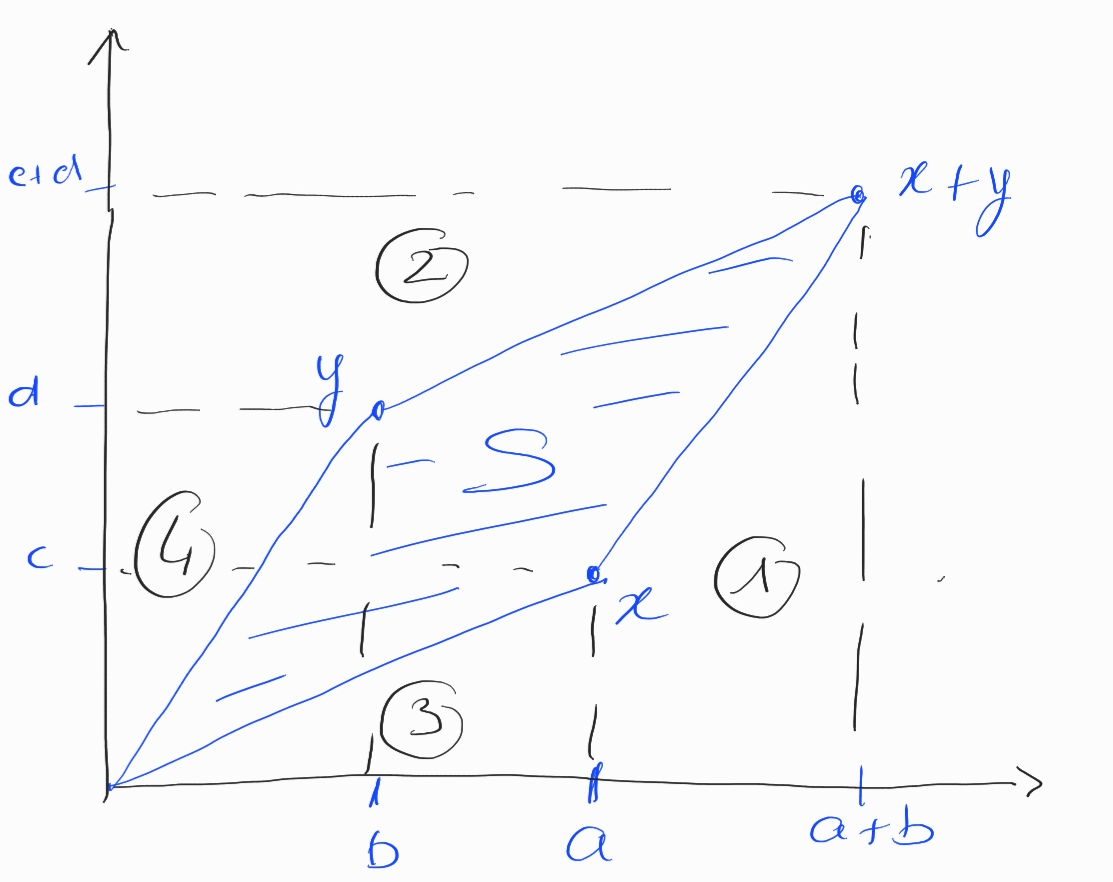
\includegraphics{DeterminantVolumeDimension2}
    $$
    soit
    \begin{align*}
      S 
      & = (a+b)(c+d) 
      - \underset{(1)}{\underbrace{b\left(c + \frac{d}2\right)}} 
      - \underset{(2)}{\underbrace{c\left(b + \frac{a}2\right)}} 
      - \underset{(3)}{\underbrace{\left(\frac{ac}2\right)}} 
      - \underset{(4)}{\underbrace{\left(\frac{bd}2\right)}} \\
      & = \dots = ad - bc.
    \end{align*}
  \item En dimension $n$ : matrice diagonale = volume d'un parallélépipède.
  \end{itemize}
\end{enumerate}

%-------------------------------------------------------------------------------
%-------------------------------------------------------------------------------
\subsection{Calcul de déterminant de matrices $n \times n$} 
%-------------------------------------------------------------------------------

On s'intéresse ici au calcul effectif d'un déterminant.

\begin{proposition}[Déterminant par blocs] \label{prop:determinantParBlocs}
  Soit $A \in \Mcal_{n,n}$ de la forme
  $$
  A = \left[\begin{array}{cc}
      B & C \\ 0_{n-p, p} & D
    \end{array}\right]
  $$
  où $1 \leq p < n$, $B \in \Mcal_{p, p}$, $C \in \Mcal_{p, n-p}$, $0_{n-p, p}$ est l'élément nul de $\Mcal_{n-p, p}$, $D \in \Mcal_{n-p, n-p}$, on a
  $$
  |A| = |B| |D|.
  $$
\end{proposition}

La proposition \ref{prop:determinantParBlocs} est donnée sans démonstration. Intuitivement, elle repose sur la formule générale du déterminant \eqref{eq:determinant} : toute permutation $\sigma$ intervertissant un des $p$ premiers éléments avec un des $n-p$ derniers fait nécessaire intervenir un élément du bloc $0_{n-p, p}$ et le produit qui lui est associé est donc nul.
\eproof

\remark Le déterminant de $A$ ne dépend donc pas des éléments de $C$.

\begin{proposition}[Déterminant d'une matrice triangulaire] \label{prop:determinantMatriceTriangulaire}
  Si $A \in \Mcal_{n,n}$ est triangulaire, 
  $$
  A = \prod_{i=1}^n a_{ii}.
  $$
\end{proposition}

% {Démonstration de la proposition \ref{prop:determinantMatriceTriangulaire}.}
\proof
En appliquant le calcul de déterminant par blocs par récurrence:
\begin{align*}
  |A| 
  & = 
  \left|\left[\begin{array}{c;{2pt/2pt}ccc}
                a_{11} & a_{12} & \dots & a_{1n} \\
                \hdashline[2pt/2pt]
                0 & a_{22} &  & a_{2n} \\
                \vdots  & \ddots & \ddots & \vdots \\
                0 & \dots & 0 & a_{nn} \\
              \end{array}\right]\right| 
  = a_{11} \times 
  \left|\left[\begin{array}{c;{2pt/2pt}ccc}
                a_{22} & a_{23} & \dots & a_{2n} \\
                \hdashline[2pt/2pt]
                0 & a_{33} &  & a_{3n} \\
                \vdots & \ddots & \ddots & \vdots \\
                0 & \dots & 0 & a_{nn} \\
              \end{array}\right]\right| \\
  & = a_{11} \times a_{22} \times 
  \left|\left[\begin{array}{c;{2pt/2pt}ccc}
                a_{33} & a_{34} & \dots & a_{3n} \\
                \hdashline[2pt/2pt]
                0 & a_{44} &  & a_{4n} \\
                \vdots  & \ddots & \ddots & \vdots \\
                0 & \dots & 0 & a_{nn} \\
              \end{array}\right]\right| 
  = \dots = a_{11} \times a_{22} \times \dots \times a_{n-1, n-1} \times a_{nn}.
\end{align*}
\eproof

\begin{definition}[Mineur et cofacteur] \label{def:mineurCofacteur}
  Pour une matrice $A \in \Mcal_n$, 
  \begin{enumerate}[\itemdot]
   \item on note $A^{(ij)}$ la matrice $A$ privée de sa $i$-ème ligne et de sa $j$-ème colonne,
   \item on appelle {\em mineur} le déterminant $|A^{(ij)}|$ et
   \item on appelle {\em cofacteur} de l'élément $(i, j)$, le produit $(-1)^{i+j} |A^{(ij)}|$.
  \end{enumerate}
\end{definition}

\begin{proposition}[Méthode des cofacteurs] \label{prop:methodeCofacteurs}
  Pour $A \in \Mcal_n$ et pour tout $i_0, j_0 \in \{1, \dots, n\}$, on a 
  \begin{align*}
    |A| 
    & = \sum_{j=1}^n a_{i_0j} (-1)^{i_0+j} |A^{(i_0j)}| & (\text{développement par rapport à la ligne $i_0$}) \\
    & = \sum_{i=1}^n a_{ij_0} (-1)^{i+j_0} |A^{(ij_0)}| & (\text{développement par rapport à la colonne $j_0$})
  \end{align*}
\end{proposition}

La démonstration de la proposition \ref{prop:methodeCofacteurs} sera faite en TD. \eproof

\remark Cette formule fournit une autre démonstration de l'équation \eqref{eq:determiantMatriceDiagonale} en développant successivement par rapport à chaque ligne : $D_n = \lambda_n D_{n-1}$.

\paragraph*{Exemples.}
\begin{itemize}
  \item Le déterminant de la matrice 
  \begin{align*}
    A_1 & = \left[\begin{array}{rrr}
      2 & -1 & 3 \\ 2 & -1 & 6 \\ -2 & 1 & 0
      \end{array}\right], &
  \end{align*}
  est nul car la première colonne est égale à $(-2)$ fois la seconde.
  \item Le déterminant de la matrice
  \begin{align*}
    A_2 & = \left[\begin{array}{rrr}
      2 & -1 & 3 \\ 2 & -1 & 6 \\ 1 & 0  & 2
      \end{array}\right]
  \end{align*}
  vaut $-3$, en développant par rapport à la dernière ligne :
  $$
  |A_2|
  = \left|\begin{array}{rrr}
    2 & -1 & 3 \\ 2 & -1 & 6 \\ 1 & 0  & 2
    \end{array}\right|
  = 1 \left|\begin{array}{rr} -1 & 3 \\ -1 & 6 \end{array}\right|
  + 2 \left|\begin{array}{rr} 2 & -1 \\ 2 & -1 \end{array}\right|
  = 1 \times (-3) + 2 \times 0 = -3.
  $$
\end{itemize}


%-------------------------------------------------------------------------------
%-------------------------------------------------------------------------------
\subsection{Inverse d'une matrice $n \times n$}
%-------------------------------------------------------------------------------

\begin{proposition} \label{prop:inverseMatriceCofacteurs}
  Soit $A \in \Mcal_n$ une matrice inversible, soit $B$ la matrice de ses cofacteurs : 
  $$
  B = [b_{ij}]_{1 \leq i, j \leq n}, \qquad 
  b_{ij} = (-1)^{i+j} |A^{(ij)}|.
  $$
  L'inverse de $A$ est égale à la transposée de la matrice de ses cofacteurs divisée par son déterminant : 
  $$
  A^{-1} = \frac1{|A|} B^\top.
  $$
\end{proposition}

% {Démonstration de la proposition \ref{prop:inverseMatriceCofacteurs}.} 
%   voir \url{https://www.techno-science.net/definition/5091.html}
\proof
La démonstration repose sur le calcul d'un élément quelconque du produit $C = A B^\top$. En notant $C = [c_{ik}]_{1 \leq i, k \leq n}$ : 
$$
c_{ik} 
= \sum_{j=1}^n a_{ij} b_{kj} 
= \sum_{j=1}^n (-1)^{j+k} a_{ij} |A^{(kj)}|.
$$
\begin{description}
  \item[$i = k$:] on reconnaît le calcul du déterminant de $A$ obtenu en développant par rapport à sa $i$-ème ligne : 
  $$
  c_{ik} 
  = \sum_{j=1}^n (-1)^{j+i} a_{ij} |A^{(ij)}|
  = |A|.
  $$
  \item[$i \neq k$:] on reconnaît $(-1)^{j+i} a_{ij} |A^{(kj)}|$ comme le déterminant, calculé par blocs, de la matrice
  $$
  \left[\begin{array}{ccccccc}
         a_{1, 1} & \cdots & a_{1,j-1} & 0 & a_{1, j+1} & \cdots & a_{1, n} \\
         \vdots & & \vdots & \vdots & \vdots &  & \vdots \\
         a_{k-1,1} & \cdots & a_{k-1,j-1} & 0 & a_{k-1, j+1} & \cdots & a_{k-1, n} \\
         0 & \cdots & 0 & a_{i, j} & 0 & \cdots & 0 \\
         a_{k+1,1} & \cdots & a_{k+1,j-1} & 0 & a_{k+1, j+1} & \cdots & a_{k+1, n} \\
         \vdots & & \vdots & \vdots & \vdots &  & \vdots \\
         a_{n, 1} & \cdots & a_{n,j-1} & 0 & a_{n, j+1} & \cdots & a_{n, n} 
        \end{array}\right]
  $$
  qui est égale à celui de la matrice
  $$
  \left[\begin{array}{ccccccc}
         a_{1, 1} & \cdots & a_{1,j-1} & a_{1, j} & a_{1, j+1} & \cdots & a_{1, n} \\
         \vdots & & \vdots & \vdots & \vdots &  & \vdots \\
         a_{k-1,1} & \cdots & a_{k-1,j-1} & a_{k-1, j} & a_{k-1, j+1} & \cdots & a_{k-1, n} \\
         0 & \cdots & 0 & a_{i, j} & 0 & \cdots & 0 \\
         a_{k+1,1} & \cdots & a_{k+1,j-1} & a_{k+1, j} & a_{k+1, j+1} & \cdots & a_{k+1, n} \\
         \vdots & & \vdots & \vdots & \vdots &  & \vdots \\
         a_{n, 1} & \cdots & a_{n,j-1} & a_{n, j} & a_{n, j+1} & \cdots & a_{n, n} 
        \end{array}\right].
  $$
  $c_{ik}$ est donc le déterminant de la matrice $A$ dont la $k$-ème ligne est remplacée par la $i$-ème ligne. 
  Cette matrice possède deux lignes égales (la $i$-ème et la $k$-ème), donc son déterminant est nul, donc $c_{ik} = 0$.
\end{description}
On a ainsi montré que
$$
c_{ik} = \left\{\begin{array}{ll} 
                  |A| & \text{si $i = k$} \\
                  0 & \text{sinon}.
                \end{array} \right.
\qquad \Leftrightarrow \qquad
C = AB^\top = |A| I
\qquad \Leftrightarrow \qquad
A^{-1} = B^\top \left/|A|\right..
$$
\eproof
